\section{How We Use the \EnergyInteractionModel{}}
\label{act2.1.4}

\begin{overview}
	\textbf{Overview:} In this activity, we reflect on what we did when using the \EnergyInteractionModel{}. We'll generate some general guidelines for successful application of the model to make sense of physical phenomena.
\end{overview}


\subsection{Reflecting on Using the \EnergyInteractionModel{}}

In the previous activities we have been applying the \EnergyInteractionModel{} to a wide range of physical phenomena. Previously, we had applied it to thermal and chemical interactions. Here is a list of what we've just done with mechanical phenomena:

\begin{itemize}
	\item \hyperref[act2.1.1]{Activity~\ref*{act2.1.1}}	Dropped golf ball and dropped coffee filter
	\item \hyperref[act2.1.2]{Activity~\ref*{act2.1.2}}	Oscillating mass attached to a spring
	\item \hyperref[act2.1.3]{Activity~\ref*{act2.1.3}} \hyperref[act2.1.3a]{Three thrown rocks}, \hyperref[act2.1.3b]{Pulling up a bucket}, and \hyperref[act2.1.3c]{Toy car launcher}
\end{itemize}

\noindent In all of these cases we used the \EnergyInteractionModel{} to make sense of the phenomena, answer questions, make predictions, or develop explanations regarding the phenomena. But the \EnergyInteractionModel{} is a very general model that needs to be refined to tell us anything about the particular phenomena.

\begin{enumerate}
	\item What did you have to do and what decisions did you have to make in order to use/apply the \EnergyInteractionModel{}? There are \textbf{three} major decisions you must initially make that determine how you are modeling the process or phenomenon. The process of making an \EnergyDiagram{} helps you with this. List the most important three things you can think of here and on your board:
	\begin{enumerate}
		\item \hrulefill
		\item \hrulefill
		\item \hrulefill
	\end{enumerate}
	
	\item Which steps on the two-page blue model summary of the \EnergyInteractionModel{} do the above three steps correspond to? \hrulefill
\end{enumerate}
	
\noindent The process of making these decisions/choices is the \textbf{\em first step} in what we have and will continue to refer to as creating or developing a \textbf{\em particular model}. This is the model that can be directly applied to a particular phenomenon.

\WCD

\subsection{The Whole Process}

\begin{enumerate}
	\item To complete the creation of the particular model, you must do some more things, perhaps make some decisions. When first encountering a phenomenon, an \EnergyDiagram{} can be particularly useful because as you draw the diagram, you are forced to make these decisions.
	
	\item Create a particular model for the case of a mass hanging on a spring that is pulled down and released at a distance ``$d$'' below the point where the mass is hanging stationary. After the mass has completed a total of 10 complete oscillations, it is noticed that it didn't go quite as far down as the distance $d$. Put your particular model, in the form of a complete \EnergyDiagram{}, on the board. Be prepared to discuss in detail the decisions you had to make when forming this diagram.
	
	\item What are some of the questions that you could ask/answer or predictions you could make with this particular model? You would likely need to have more specific information that you could obtain from the phenomenon. Put these questions on the board with any additional information you would need.
\end{enumerate}

\WCD

\subsection{A New Phenomenon}

Imagine this situation: Two {\em identical} balls roll down two sets of slanted channels. The slope and length of the channels are the {\em same}, so the change in height is the same for both balls. However, the channels have different widths: one is wider than the other.

\begin{center}
	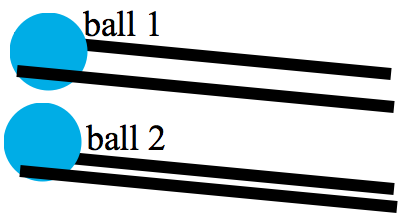
\includegraphics[width=0.25\textwidth]{act214-ramps}
\end{center}

\noindent Your instructor will give you two Pool balls. Let them roll down the channels -- starting them at the same time -- and observe what happens. Do this several times, carefully observing what is different about the way the balls roll. Could the difference be an indication that there is a new energy system that we need to take into account?

A maybe obvious question is, \textbf{\emph{``Why does one ball go faster and get to the bottom before the other ball?''}} Use the \EnergyInteractionModel{} to make sense of what is going on, and develop a succinct explanation with an appropriate \EnergyDiagram{} for why one of the balls gets to the bottom of the rails before the other ball.

\textbf{Note:} From careful measurements made on this apparatus, friction plays only a very small roll in the difference in speeds of the balls. You can safely assume that all frictional effects cause negligible energy changes compared to the changes in mechanical energies. 

\WCD